\documentclass[../CSC_5RO17_TA_TP1.tex]{subfiles}

\begin{document}
\subsection*{Question 1}
\begin{definition}
    Une \textbf{Homographie} est une transformation projective entre deux plans $\pi_1$ et $\pi_2$ qui conserve les lignes droites. Une \textbf{Homographie} peut-être represente par l'équation suivant:
    \begin{equation}
        \boxed{
            \begin{bmatrix}
            x_2\\ y_2\\ 1
            \end{bmatrix}
            =
            \underbrace{
                \begin{bmatrix}
                    a_{11} & a_{12} & t_x\\
                    a_{21} & a_{22} & t_y\\
                    v_1    & v_2    & 1\\
                \end{bmatrix}
            }_{\text{Homographie}}
            \times
            \begin{bmatrix}
                x_1\\ y_1\\ 1
            \end{bmatrix}
        }
    \end{equation}
\end{definition}
\noindent En termes simples, cela signifie que si deux images d'une scène sont prises sous certaines conditions géométriques, la relation entre ces images peut être modélisée par une \textbf{Homographie}. Cas où la transformation est une homographie:
\begin{enumerate}[noitemsep, rightmargin=\leftmargin]
    \item images d'un même plan vu sous deux poses 3D différentes;
    \begin{figure}[H]
        \centering
        \includegraphics[width=100mm, page=25]{../CSC_5RO17_TA cours_homographie.pdf}
        \caption{Différent 3D poses}
        \label{fig_2_3d_positions}
    \end{figure}
    \item images prises par une caméra tournant autour de son centre optique;
    \begin{figure}[H]
        \centering
        \includegraphics[width=100mm, page=24]{../CSC_5RO17_TA cours_homographie.pdf}
        \caption{Rotation centre optique}
        \label{fig_rotation_optical_center}
    \end{figure}
\end{enumerate}
\end{document}
